\section{Auswertung der Daten}
Für die Auswertung der Daten werden im Folgenden die Pakete \textit{pandas} \cite{pandas}, \textit{numpy} \cite{numpy} und \textit{sklearn} \cite{sklearn} verwendet, während die Plots durch das Paket \textit{matplotlib.pyplot} \cite{matplotlib} erstellt werden.

\subsection{Vorbereitung}
Aus den Daten werden zu Beginn sowohl die Features entfernt, welche nicht in beiden Datensätzen zu finden sind, als auch die Features, welche Monte-Carlo-Wahrheiten, Identifikationsnummern oder Gewichte repräsentieren. Für das Letztere werden die Features mit den Stichworten
\begin{itemize}
    \item Corsica
    \item MC
    \item Weight
    \item ID
    \item Header
    \item SPline
\end{itemize}
aus den Datensätzen entfernt. Übrig bleiben 188 Attribute, welche für die Lerner genutzt werden können.

Des Weiteren werden alle Einträge, welche ein $NaN$ oder $Inf$ enthalten, durch den Wert $-5000$ ersetzt. Es kann angenommen werden, dass dieser Wert nicht auf natürliche Weise durch die simulierten Daten erreicht wird.

Die Daten werden im Anschluss durch die Zahlen 0 und 1 gelabelt, wobei die Zahl null für den Untergrund und die Zahl eins für das Signal verwendet wird.

Der Datensatz wird zudem mit der Funktion \textit{StandardScaler} skaliert.

\subsection{Auswahl der Attribute}
Die Features für die Lerner werden mit Hilfe einer Forward-Selection ausgewählt. Es wird die Implementierung \textit{SelectKBest} von \textit{sklearn.feature\_selection} verwendet. 

Um starke statistische Schwankungen bei der Auswahl der Features zu vermeiden, wird der Jacccard-Index nach Abschnitt \ref{jaccard} berechnet und in Abhängigkeit von der Feature-Anzahl in Abbildung \ref{fig:jaccard} dargestellt. Hierzu wird der Datensatz in fünf gleichgroße Teile gesplittet und auf jedem Teil die Featureselektion durchgeführt. Anschließend wird für jede Kombination der Datensätze der Jaccard-Index als Maß für die Ähnlichkeit der Featuremengen ermittelt und nach \eqref{eq:jc} aufsummiert.
\begin{figure}
  \centering
  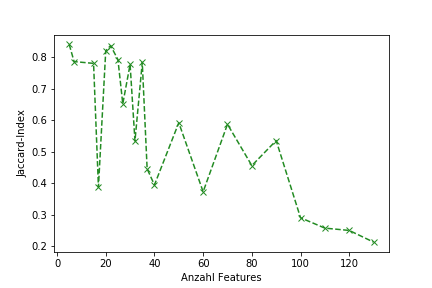
\includegraphics[width=0.7\textwidth]{plots/jaccard.png}
  \caption{Jaccard-Index der selektierten Features zur Untersuchung der statistischen Schwankungen.}
  \label{fig:jaccard}
\end{figure}
\FloatBarrier
Es lässt sich ein Plateu in einem Bereich von 20 bis 40 Features erkennen. Um eine stabile Auswahl zu gewährleisten, sollte die Anzahl der ausgewählten Features in diesem Bereich liegen. Da aber auch andere Parameter bei der Auswahl eine Rolle spielen, wird die Anzahl der Features im Folgenden zunächst im Intervall von 20 bis 150 in Zehnerschritten varriiert.

Im Anschluss wird der Datensatz mittels \textit{train\_test\_split} in einen Test- und einen Trainingsdatensatz aufgeteilt. Hierbei werden $\SI{30}{\%}$ des Datensatzes zum Testen verwendet.

\subsection{Random-Forest-Klassifikator}
Als erster Lerner wird ein Random-Forest-Modell über die Funktion \textit{RandomForestClassifier} von \textit{sklearn.ensemble} mit einer Baumanzahl von 100 erstellt, die Lerndatensätze mit verschiedenen Featureanzahlen trainiert und anschließend die Klassen der Testdatensätze vorhergesagt. Aus diesen Informationen werden anschließend die Reinheit mittels der Funktion \textit{accuracy\_score}, die Effizienz mittels \textit{precision\_score}, der Jaccard-Index mittels \textit{jaccard\_similarity\_score} und die Fläche unter der ROC-Kurve mit der Funktion \textit{roc\_auc\_score} nach den Zusammenhängen aus Kapitel \ref{kap:Theorie} berechnet und in Abhängigkeit von der Featureanzahl in Abbildung \ref{fig:RF_Feat} abgebildet.
\begin{figure}
    \centering
    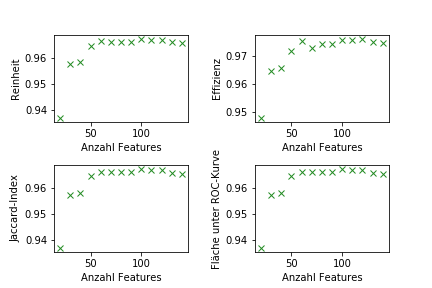
\includegraphics[width=0.7\textwidth]{plots/RF_featurezahl.png}
    \caption{Qualitätsparameter der Random-Forest-Klassifizierung in Abhängigkeit von der Featureanzahl. Von links oben: Reinheit, Effizienz, Jaccard-Index und Fläche unter der ROC-Kurve.}
    \label{fig:RF_Feat}
  \end{figure}
  \FloatBarrier
  Alle vier Parameter steigen zu Beginn um etwa zwei Prozentpunkte an und gehen dann anschließend in eine Sättigung über. Als beste Featureanzahl wird der erste Wert im Sättigungsbereich verwendet, welcher durch den Wert 40 gegeben ist. Für diese wird die Random-Forest-Klassifizierung erneut für zehn verschiedene Baumanzahlen im Bereich von 10 bis 100 durchgeführt. Die Qualitätsparameter für die unterschiedlichen Baumzahlen sind Abbildung \ref{fig:RF_Tiefe} zu entnehmen.
  \begin{figure}
    \centering
    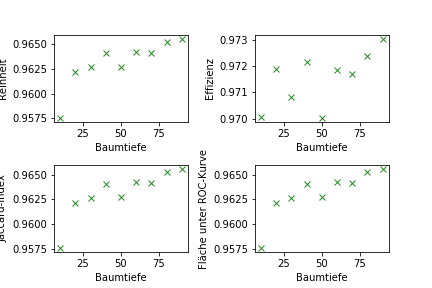
\includegraphics[width=0.7\textwidth]{plots/RF_baumtiefe.png}
    \caption{Qualitätsparameter der Random-Forest-Klassifizierung in Abhängigkeit von der Baumanzahl. Von links oben: Reinheit, Effizienz, Jaccard-Index und Fläche unter der ROC-Kurve.}
    \label{fig:RF_Tiefe}
  \end{figure}
  \FloatBarrier
  Es lässt sich erkennen, dass die Baumanzahl lediglich einen sehr geringen Einfluss von weniger als einen Prozentpunkt auf die Qualitätsparameter hat. Um Rechenzeit zu sparen wird deshalb im Folgenden eine minimale Baumanzahl von 10 verwendet.

  Für die gefundenen Parameter wird eine Cross-Validation durchgeführt. Hierzu wird die Funktion \textit{cross\_val\_score} genutzt und der Datensatz in 5 Teile gesplittet.
  Die gefundenen Qualitätsparameter sind in Tabelle \ref{tab:RF} dargestellt und werden über die 5 Durchläufe gemittelt.
  \begin{table}[ht]
    \centering
    \caption{Qualitätsparameter der Cross-Validation für den Random-Forest-Klassifikator.}
    \label{tab:RF}
    \sisetup{table-format=2.1}
    \begin{tabular} { c | c c c}
    \toprule
    {} & {Reinheit} & {Effizienz} & {AUC} \\
    \midrule
        & 0.914 & 0.881 & 0.975 \\
       & 0.955 & 0.975 &  0.989\\
       & 0.961 & 0.984 &  0.992\\
       & 0.960 & 0.985 &  0.991 \\
       & 0.962 & 0.985 &  0.994 \\
    \midrule
      Mittelwert & 0.950 \pm 0.009 & 0.962 \pm 0.020 &  0.988 \pm 0.003 \\
    \bottomrule
    \end{tabular}
    \end{table}
    \FloatBarrier
Zuletzt wird die Vorhersagekraft des besten Random-Forest-Modells in einer sogenannten Confusion-Matrix (deutsch: Wahrheits-Matrix) dargestellt. Diese stellt die Rate der richtig bzw. falsch zugeordneten Klassen dar. Das Label 0 repräsentiert hierbei den Untergrund und der Wert 1 das Signal. 
Der Lerner ordnet das Ereignis der Klasse zu, welche die höhere Wahrscheinlichkeit besitzt. Dieses entspricht einem Konvidenzschnitt von 0.5.
Die Matrix wird über die Funktion \textit{confusion\_matrix} berechnet und über die Funktion \textit{plot\_confusion\_matrix} nach \textit{sklearn} geplottet. Die Confusion-Matrix für den Random-Forest-Klassifikator ist in Abbildung \ref{fig:RF_Conf} zu sehen.
\begin{figure}
    \centering
    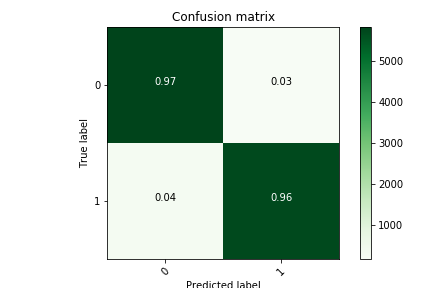
\includegraphics[width=0.7\textwidth]{plots/RF_confusion.png}
    \caption{Confusion-Matrix für den Random-Forest-Klassifikator mit einer Tiefe von 10 und einer Featureanzahl von 40 (0: Untergrund, 1: Signal).}
    \label{fig:RF_Conf}
  \end{figure}
  \FloatBarrier

  \subsection{kNN-Klassifikator}
  Das kNN-Klassifikator-Modell wird mittels der Funktion \textit{KNeighborsClassifier} von \textit{sklearn.neighbors} erstellt. Für eine Nachbaranzahl von 10 werden zunächst analog zum Random-Forest-Klassifikator die Qualitätsparameter für unterschiedliche Featureanzahlen ermittelt und in Abbildung \ref{fig:kNN_feat} dargestellt.
  \begin{figure}
    \centering
    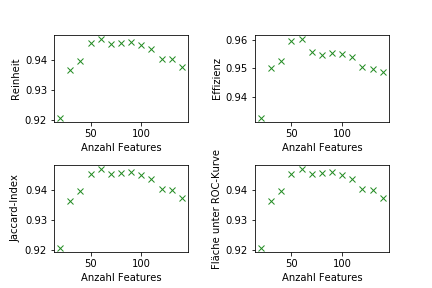
\includegraphics[width=0.7\textwidth]{plots/kNN_featurezahl.png}
    \caption{Qualitätsparameter der kNN-Klassifizierung in Abhängigkeit von der Featureanzahl. Von links oben: Reinheit, Effizienz, Jaccard-Index und Fläche unter der ROC-Kurve.}
    \label{fig:kNN_feat}
  \end{figure}
  \FloatBarrier
Es lässt sich eine Schwankung um etwa zwei Prozentpunkte mit einem klaren Maximum bei einer Featureanzahl von 50 erkennen. Dieser Wert wird im Folgenden als Bestwert verwendet.
Außerdem werden die Qualitätsparameter erneut in Abhängigkeit von der Anzahl an nächsten Nachbarn ermittelt und in Abbildung \ref{fig:kNN_nachbarn} aufgetragen. Die Nachbaranzahl wird hierbei von 10 bis 100 in Zehnerschritten varriiert.
\begin{figure}
    \centering
    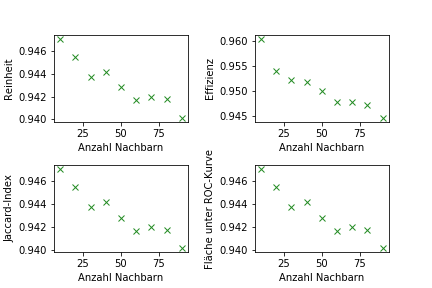
\includegraphics[width=0.7\textwidth]{plots/kNN_nachbarzahl.png}
    \caption{Qualitätsparameter der kNN-Klassifizierung in Abhängigkeit von der Anzahl an Nachbarn. Von links oben: Reinheit, Effizienz, Jaccard-Index und Fläche unter der ROC-Kurve.}
    \label{fig:kNN_nachbarn}
  \end{figure}
  \FloatBarrier
Es lässt sich ein kontinuierlicher Abfall der Werte mit der Anzahl der Nachbarn um etwa einen halben Prozentpunkt beobachten. Aus diesem Grund wird als bester Fall die Nachbaranzahl 10 festgelegt.
Im Anschluss wird analog zum vorherigen Unterkapitel eine Cross-Validation für das beste Modell durchgeführt. Die Ergebnisse sind in Tabelle \ref{tab:kNN} abgebildet.
\begin{table}[ht]
    \centering
    \caption{Qualitätsparameter der Cross-Validation für den kNN-Klassifikator.}
    \label{tab:kNN}
    \sisetup{table-format=2.1}
    \begin{tabular} { c | c c c}
    \toprule
    {} & {Reinheit} & {Effizienz} & {AUC} \\
    \midrule
        & 0.886 & 0.854 & 0.961 \\
       & 0.945 & 0.958 &  0.985\\
       & 0.953 & 0.976 &  0.988\\
       & 0.952 & 0.977 &  0.987 \\
       & 0.953 & 0.978 &  0.988 \\
    \midrule
      Mittelwert & 0.938 \pm 0.013 & 0.949 \pm 0.024 &  0.982 \pm 0.005 \\
    \bottomrule
    \end{tabular}
    \end{table}
    \FloatBarrier
Die Confusion-Matrix für das beste Modell ist in Abbildung \ref{fig:kNN_conf} zu erkennen.
\begin{figure}
    \centering
    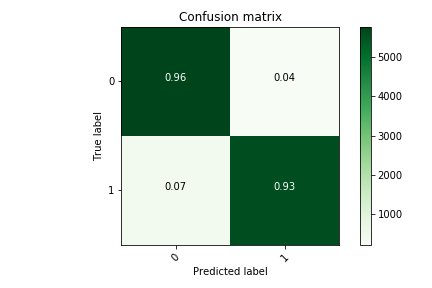
\includegraphics[width=0.7\textwidth]{plots/kNN_confusion.png}
    \caption{Confusion-Matrix für den kNN-Klassifikator mit einer Nachbaranzahl von 10 und einer Featureanzahl von 50 (0: Untergrund, 1: Signal).}
    \label{fig:kNN_conf}
  \end{figure}
  \FloatBarrier

\subsection{Naive-Bayes-Lerner}
Als dritter Klassifikator wird ein Naive-Bayes-Lerner über die Funktion \textit{GaussianNB} von \textit{sklearn.naive\_bayes} verwendet. Analog zu den vorherigen Kapiteln werden zunächst erneut die Qualitätsparameter in Abhängigkeit von der Featureanzahl ermittelt und in Abbildung \ref{fig:NB_feat} dargestellt.
\begin{figure}
  \centering
  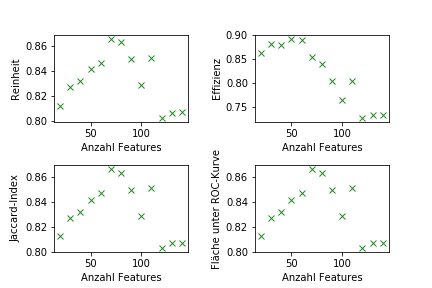
\includegraphics[width=0.7\textwidth]{plots/NB_featurezahl.png}
  \caption{Qualitätsparameter der Naive-Bayes-Klassifizierung in Abhängigkeit von der Featureanzahl. Von links oben: Reinheit, Effizienz, Jaccard-Index und Fläche unter der ROC-Kurve.}
  \label{fig:NB_feat}
\end{figure}
\FloatBarrier
Die Werte steigen zunächst kontinuierlich an und nehmen ein Maximum bei $k_{\mathrm{NB}} = 60$ an. Anschließend fallen sie mit einigen Schwankungen wieder ab. Der maximale Wert wird als Bestwert für die Featureanzahl festgelegt. 
Anschließend wird erneut eine Cross-Validation durchgeführt und die Ergebnisse in Tabelle \ref{tab:NB} aufgeführt.
\begin{table}[ht]
  \centering
  \caption{Qualitätsparameter der Cross-Validation für den Naive-Bayes-Klassifikator.}
  \label{tab:NB}
  \sisetup{table-format=2.1}
  \begin{tabular} { c | c c c}
  \toprule
  {} & {Reinheit} & {Effizienz} & {AUC} \\
  \midrule
      & 0.805 & 0.764 & 0.862 \\
     & 0.795 & 0.720 &  0.922\\
     & 0.867 & 0.855 &  0.938\\
     & 0.861 & 0.844 &  0.935 \\
     & 0.870 & 0.867 &  0.939 \\
  \midrule
    Mittelwert & 0.840 \pm 0.016& 0.810 \pm 0.029 &  0.919 \pm 0.015 \\
  \bottomrule
  \end{tabular}
  \end{table}
  \FloatBarrier
  Die Confusion-Matrix für den Naive-Bayes-Lerner ist in Abbildung \ref{fig:NB_conf} zu sehen.
  \begin{figure}
    \centering
    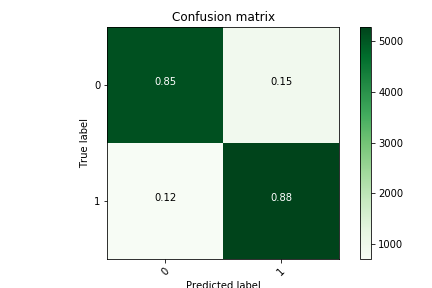
\includegraphics[width=0.7\textwidth]{plots/NB_confusion.png}
    \caption{Confusion-Matrix für den Naive-Bayes-Klassifikator mit Featureanzahl von 60 (0: Untergrund, 1: Signal).}
    \label{fig:NB_conf}
  \end{figure}
  \FloatBarrier

  \subsection{Zusammenfassung}
  In Abbildung \ref{fig:roc} ist die ROC-Kurve für die besten Modelle der drei verwendeten Lerner abgebildet. Hierzu wird die Funktion \textit{roc\_curve} von \textit{sklearn.metrics} verwendet. Für eine ideale Trennung der Klassen, würde die Kurve parallel zur $y$-Achse auf den Wert $1$ ansteigen und anschließend parallel zur $x$-Achse verlaufen. Für den Fall, dass die Klassen nur sehr schlecht voneinander getrennt werden können, hat die ROC-Kurve die Form einer Diagonalen durch den Nullpunkt.
  \begin{figure}
    \centering
    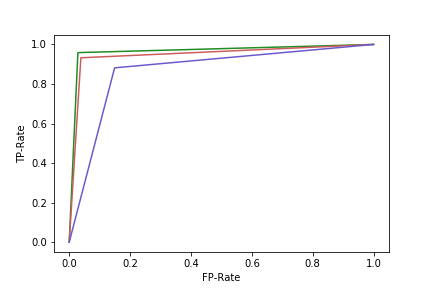
\includegraphics[width=0.7\textwidth]{plots/roc_kurve.png}
    \caption{ROC-Kurve für die besten Modelle des Random-Forest-Klassifikators (grün), des kNN-Klassifikators (rot) und des Naive-Bayes-Lerner (blau). Für einen idealen Klassifiaktor wird für alle $x$- Werte zwischen null und eins der $y$-Wert eins angenommen.}
    \label{fig:roc}
  \end{figure}
  \FloatBarrier
